\documentclass[a4paper]{article}
\usepackage{graphicx}
\usepackage{twocolpceurws}
\usepackage[utf8]{inputenc}
\usepackage{enumitem}
\usepackage{color}
\usepackage{amsmath}

\newcommand{\cn}[1]{\textsuperscript{\color{red} ~[citation needed](#1)~}}

\title{Measuring the impact of library dependency on maintenance}

\author{
Núria Bruch Tàrrega \\ University of Amsterdam \\ nuria.bruchtarrega@student.uva.nl
\and
Miroslav \v{Z}ivkovi\'{c} \\ Software Improvement Group \\ m.zivkovic@sig.eu
\and
Ana Oprescu \\ PCS, SNE, Informatics Institute\\
                University of Amsterdam \\ a.m.oprescu@uva.nl
}

\institution{}

\begin{document}
\maketitle

\begin{abstract}

%The application developers are using open source software (OSS) libraries at an ever increasing rate nowadays. On one-hand side, this reduces time-to-market as there is no need to re-implement the functionality offered by OSS. On the other-hand side, this introduces either direct or transitive {\bf dependencies}, and
%the application developers need to manage these dependencies.

%In case when OSS library contains a security vulnerability, this vulnerability could lead to a failure of confidentiality, integrity, or availability of the product. Further, dependencies are typically declared when  an application is built using package managers. These managers will perform only a binary evaluation of the dependencies. Finally, a number of libraries in an OSS ecosystem may not be maintained for a (relatively) long time.

%Therefore, application developers may need to replace libraries used. This replacement requires an {\em effort } from the application developers, as well as the information about the respective dependencies for considered libraries.

Reusing code from open-source libraries is a useful practice for developers to avoid implementing the same functionalities multiple times. However, when a library is used in another software product, it creates a dependency that may spread the security vulnerabilities of the library to the product. Most package managers have dependency managers which only perform a binary evaluation of the dependencies. Thus, developers have no information about how much products depend on a library or how much effort would be needed to replace a dependency.

In this research, we propose a way to measure the degree of library dependency, as well as how much effort would be required to replace the usage of a library with another one. We leverage existing coupling metrics and revisit them in the context of library dependencies.

We present two metrics to measure the coupling generated by dependencies: method invocation and aggregation coupling, and briefly discuss the next steps.

%Our immediate next steps are evaluating the set of metrics and extending it to transitive dependencies.
\end{abstract}


\section{Introduction}

There are many open-source software (OSS) libraries available for the developers to reuse the features that these libraries implement \cite{kikas2017structure}. This practice allows the reuse of previously developed code and, therefore, helps developers to avoid implementing the same functionalities multiple times.

When an open-source library is used in a software product, a dependency between the product and the library is created. This adds the task of managing these dependencies to the maintenance tasks of the product, and this task is not a trivial one.
%maintenance of the dependencies is not a trivial task, and it is one of the challenges that the field of software engineering is trying to solve.

Open-source libraries can have security vulnerabilities that may affect the products that depend on these libraries. For example, some security vulnerabilities can have a negative impact in terms of integrity, privacy, or availability.

Currently, developers have package managers at their disposal, to ease the task of managing the dependencies of their products. However, these package managers only evaluate whether a dependency exists or not and a more detailed risk evaluation is missing \cite{hejderup2018prazi}. There is no way to evaluate how much a product depends on a library.

Furthermore, the developers of a project may decide to replace one of the dependencies of the product with another one. This could happen when a library has vulnerabilities or is deprecated,
%to prevent the vulnerabilities from affecting the project.
However, replacing a dependency could be a costly process. For example, it may involve identifying which parts of the project are affected by the dependency, and which parts of the library are being used and need replacement.

This work has the goal of measuring the degree of library dependency and understanding how it affects the maintenance effort. A set of metrics is proposed to measure the dependencies between software products and the open-source libraries. In addition, we propose a way to measure the effort that would be required to replace a dependency with a new one. We define a method to estimate effort considering parts of the code affected by the dependency.

\subsection{Research questions}
Based on our problem statement, we define the following research questions:

\begin{description}[noitemsep,leftmargin=*]
  \item [\textbf{RQ1:}] \textit{How can we measure the degree of source code dependency between the two libraries?}

  The goal of this research question is to define the metrics to measure dependency. We focus on coupling metrics, which have been used for many years, in particular for Object-Oriented systems \cite{briand1999unified}. The key difference is that these metrics have been used to measure coupling within a software product, and not between different software products. Therefore, the definition of coupling is changed, and so is the meaning of the metrics.

  \item [\textbf{RQ2:}] \textit{How can we measure the effort required to replace a dependency with a different one?}

  The goal of this question is to propose a methodology to estimate the effort needed to change the usages of a library. To do so, we analyze the different options to perform this replacement, and study how these affect the code. Then, we study the different methodologies available to estimate the effort, and how these would fit in this use case.
\end{description}

In what follows, we focus on RQ1.

\section{Background}\label{section:Background}
Coupling is defined  as the strength of the connection from one item to another, and is related to the maintainability of a software product \cite{gupta2009package}. To evaluate the connection or dependency between items that belong to the same product, a wide variety of metrics has been proposed to measure coupling.
There are six main groups of coupling metrics: structural, dynamic, evolutionary and logical, information entropy approach, conceptual, and domain-specific  \cite{poshyvanyk2006conceptual}. The most largely studied by the literature is the structural coupling, and it is the type of coupling measured in this research.

Briand et al. \cite{briand1999unified} defined a unified framework for coupling metrics, based on three previously existing frameworks \cite{eder1994coupling,hitz1995measuring,briand1997investigation}. They specify six criteria that define the type of coupling used for metric calculation.

\begin{description}[noitemsep,leftmargin=*]
    \item [Criterion 1:] Type of connection, which is the connection mechanism that creates coupling.
    \item [Criterion 2:] Locus of impact, the point of view from which the coupling being measured: the one that uses another element - the client (import), or the one that is being used - the server (export).
    \item[Criterion 3:] The granularity of the measure, which includes two aspects: the aggregation level (e.g. method, class, system), and how the metric counts the connections between the two elements (e.g. count each connection individually or binary evaluation of the connection between two elements).
    \item [Criterion 4:] The stability of the server, a stable server is not subject to modifications in the project at hand.
    \item [Criterion 5:] Direct/Indirect coupling, if the metric accounts for indirect relationships, or only measures the direct ones.
    \item [Criterion 6:] Inheritance, this criterion specifies how certain cases related to inheritance (e.g. inheritance and polymorphism) affect coupling.
\end{description}

\section{Related Work}
To the best of our knowledge, no studies measure the degree of dependency between libraries. However, some studies perform an evaluation of the dependencies according to certain characteristics.

Soto-Valero et al. \cite{soto2020comprehensive} conducted a study of bloated dependencies. Bloated dependencies, either direct or transitive, are those specified in the dependency set of a project, that are not used for either compilation or product deployment. The authors developed the tool \textit{DepClean}, which analyses the dependencies of Java artifacts. This tool identifies bloated dependencies and generates an alternative dependency set without bloated dependencies. Further, \textit{DepClean} creates a call-graph of the API members of the libraries and dependencies. However, the focus is on the bloated dependencies, not on measuring the degree of the dependencies.

Pashchenko et al. \cite{pashchenko2018vulnerable} propose a method to analyze dependencies in which they distinguish between own and third-party libraries, as well as deployed and non-deployed dependencies. In addition, they remark the importance of halted dependencies, since the libraries that create these dependencies are no longer updated. However, Pashchenko et al. do not perform a call-level analysis of the dependencies, since their dependency resolution is based only on the \textit{POM} file of the libraries. Hence, the transitive dependencies that are not really used in the studied library are still counted.

\section{Definition of coupling}\label{section:defCoupling}
The first step towards creating a model to measure the dependencies between libraries is to define which meaning of coupling is involved in these dependencies. Therefore, we use the framework explained in section \ref{section:Background}, from Briand et al. \cite{briand1999unified}.

\subsection{Criterion 1: Type of connection}
With this criterion, it is defined which type of connection creates coupling between the two libraries. There are several clearly distinguished mechanisms that can create coupling \cite{briand1999unified}, and are listed below.

Given class \textit{a} that belongs to library \textit{A}, and class \textit{b} that belongs to library \textit{B}...

\begin{enumerate}[noitemsep,leftmargin=*]
  \item ... class \textit{a} has an attribute of type \textit{b} (Relationship of aggregation).
  \item ... method of class \textit{a} has a parameter of type \textit{b} or has return type \textit{b}.
  \item ... method of class \textit{a} has a local variable of type \textit{b}.
  \item ... method of class \textit{a} calls a method which has a parameter of type \textit{b}.
  \item ... method of class \textit{a} references attribute of class \textit{b}.
  \item ... method of class \textit{a} invokes method of class \textit{b}.
  \item ... class \textit{a} and class \textit{b} have a relationship such as \textit{uses} or \textit{consists-of}.
\end{enumerate}

Having a single metric that measures more than one of these types of connections is not recommended as this requires to figure out if every type of connection creates the same coupling, and whether it affects maintenance in the same way. It would not be possible to know how much of the coupling is created by which type of connection.

%Therefore, all chosen types of connections are going to be measured by different metrics.
Therefore, different metrics should be used for different connections.
To decide which types of connections to measure, %since all of them create coupling between libraries,
we have decided to review the literature on coupling metrics, to understand which connections are the most measured and why.

\begin{table}[ht!]
    \centering
    \begin{tabular}{|l|c|c|c|c|c|c|c|}
         \hline
         Reference                      & 1 & 2 & 3 & 4 & 5 & 6 & 7 \\\hline
         \cite{eder1994coupling}        & x & x & x & x &   & x & x \\\hline
         \cite{hitz1995measuring}       & x & x & x &   & x & x & x \\\hline
         \cite{briand1997investigation} & x & x &   &   &   & x &   \\\hline
         \cite{wilkie2000coupling}      & x & x &   &   &   &   &   \\\hline
         \cite{yang2005detecting}       & x & x & x & x &   & x &   \\\hline
         \cite{gui2007ranking}          & x &   &   &   & x & x &   \\\hline
         \cite{gupta2009package}        & x & x & x & x & x & x & x \\\hline
         \cite{harrison1998coupling}    &   &   &   &   & x & x &   \\\hline
         \cite{du2004refactoring}       & x &   &   &   & x & x &   \\\hline
         \cite{koetter2019assessing}    & x &   &   &   & x & x &   \\\hline
    \end{tabular}
    \caption{Literature usage of the types of connection}
    \label{tab:type-con-literature}
\end{table}

 Types 1 and 6 are the most used in the literature and therefore we define a metric to measure \textbf{type 6: method invocation}.
 %It is the type of connection mostly used by coupling metrics, which have been largely reused in the literature, and reviewed and classified according to the framework by Briand et al. \cite{briand1999unified}.

The second metric that we consider is \textbf{type 1: aggregation coupling}, for two main reasons. It is used as type 6 in the reviewed literature, and because in some cases, measuring type 6 may not be enough to understand how much maintenance a library dependency may need. There is the possibility that a class has an attribute of another class, but never calls a method that belongs to that class.

The above-mentioned metrics are those that we initially consider in our work, and we will explain them in greater detail in Section~\ref{section:metrics}. Nevertheless, it might be necessary to include additional metrics, %more,
to account for other connection types.

\subsection{Criterion 2: Locus of impact}
%According to the description of the problem,
The goal of this measurement is to know how much a library depends on another. Therefore, the point of view of this evaluation is from the library that uses another one. Hence, the locus of impact of the coupling to be measured %in this work
is \textbf{import}.

\subsection{Criterion 3: Granularity of the measure}
%In this criterion,
There are two aspects to define: (1) the aggregation level of the measure, and (2) how the metric counts the connections.
First, we are going to discuss the aggregation level. Briand et al. define the following levels: Attribute, Method, Class, Set of classes, System.

%In this case, the
Our goal is to measure the coupling between the set of classes of the client library and the set of classes of the server library. %However,
In order to maintain consistency, we rename the aggregation level set of classes as \textbf{library} for the rest of the paper. To maintain the precision of the measurement, the calculation of coupling for a more coarse-grained level, such as library, is done by aggregating the coupling of the more fine-grained aggregation levels, such as method and class.

%Next, we define how the metrics count the connections.
There are two basic options for counting connections: A) counting individual connections, and B) count the different items at the other end of the connection. From a maintenance point of view, it matters whether a method is called once or multiple times, and we therefore use option A.
To support fine-grained analysis, connections are counted from the smallest aggregation level, and aggregated up to the considered aggregation level.
For example, when counting method invocations, we  \textbf{add up the number of method invocations per each method of each class of a library}.
%when a method is called only once or multiple times, it makes a difference, therefore we will use option A. In order to maintain a fine-grained analysis, the connections will be counted starting with the smallest aggregation level according to the type of connection, and aggregated across aggregation levels until the aggregation level of the metric. For example, when counting method invocations, we  \textbf{add up the number of method invocations per each method of each class of a library}.

\subsection{Criterion 4: Stability of the server}
Briand et al. \cite{briand1999unified} define stable classes as \textit{"Classes that are not subject to change in the project at hand"}. Therefore, we measure coupling from non-stable classes to stable classes.
However, the separation between stable and unstable classes is not enough. The goal is to measure coupling only with those \textbf{stable classes} that are part of third-party open-source libraries.

\subsection{Criterion 5: Direct and indirect coupling}
To make a decision about this criterion, we need to distinguish two alternative scenarios in which we want to measure coupling: direct dependencies and transitive dependencies. For the initial approach, we  focus on the direct dependencies only. Therefore, the metrics measure \textbf{direct coupling}.

\subsection{Criterion 6: Inheritance}
Within this criterion, there are three aspects to decide about: how, if at all, does the metric distinguish between inheritance-based coupling and non-inheritance-based coupling? Does the metric account for polymorphism? And finally, what determines whether a method or attribute is part of a class or not?

\begin{figure}[ht]
\begin{center}
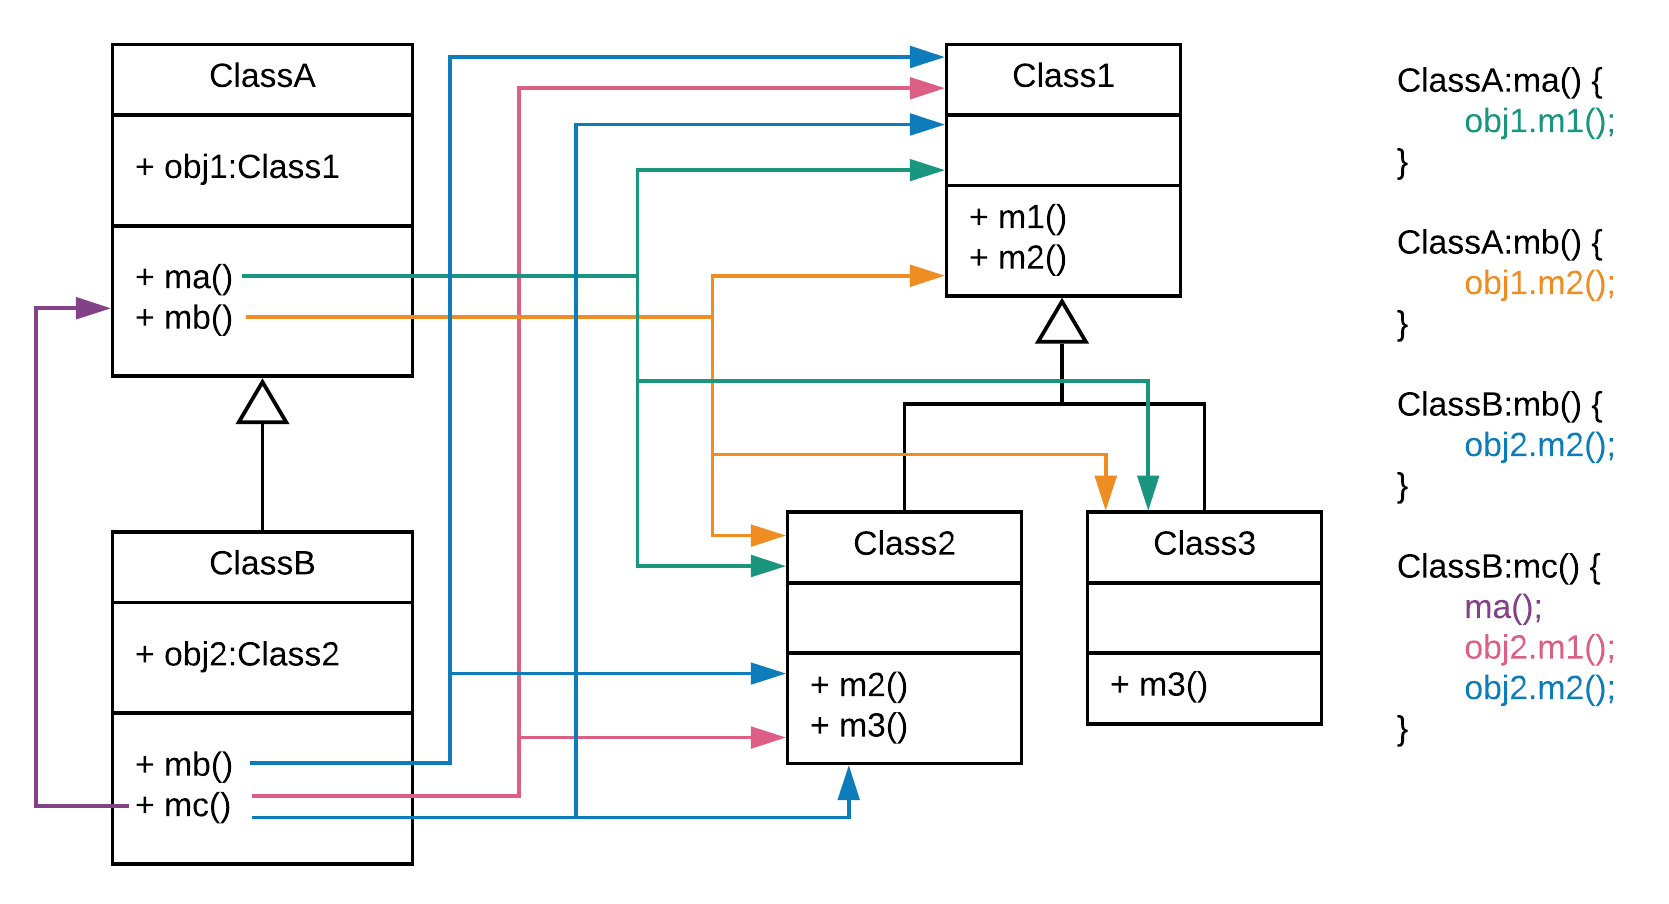
\includegraphics[height=4.4cm]{img/specialcases.png}
\caption{Example of coupling special cases, based on example from Briand et al. \cite{briand1999unified}}
\label{fig:specialcases}
\end{center}
\end{figure}

In order to answer the first question, we focus on the method \texttt{mc} of \texttt{ClassB} in Figure \ref{fig:specialcases}. This method invokes \texttt{ma} of \texttt{ClassA}, inherited by a class \texttt{ClassB}.
%a class from which \texttt{ClassB} inherits.
This %is known as
{\em inheritance-based} coupling is sometimes considered as a special case of coupling. %Should this connection be considered as a special case and be counted separately from the rest when considering maintenance effort?
When there is a change of an inherited method that a class uses, it  requires the same maintenance effort as the method that is not inherited. Therefore, our metrics  \textbf{include inheritance-based coupling without distinction}.

%Next, we discuss about whether to account for polymorphism.
In case of polymorphism we look at the methods of \texttt{ClassA}. This class contains an attribute of type \texttt{Class1},
%which considering dynamic assignation of types could also be of type
which could be of type \texttt{Class2} or \texttt{Class3}.
%In this case,
We first analyze whether a call to a method of \texttt{Class1} would create coupling with \texttt{Class2} and \texttt{Class3}, and if it makes a difference when the method is overridden or not. The method \texttt{ma} invokes \texttt{m1}, which is not overridden by any of the descendants of \texttt{Class1}. When a change is made in \texttt{Class2} or \texttt{Class3} no change is required as the invoked method remains the same. In contrast, method \texttt{mb} calls \texttt{m2}, which is overridden in \texttt{Class2}. Here, the implementation of \texttt{m2} in \texttt{Class2} could be updated, and this may affect the way \texttt{ClassA} uses it, and therefore changes may be needed. Thus, %we consider that
it is necessary to \textbf{account for polymorphism}.

%Lastly, we discuss about how do decide if a method belongs or not to a
%class. We have two options:
Further, a method belongs to the class that implements it (could be more than one since we account for polymorphism), or a method belongs to the class that it is referenced from. %An example of this can be found in
The last two lines of the method \texttt{mc} of \texttt{ClassB} call method \texttt{m1} and \texttt{m2} on an object of type \texttt{Class2}. The difference is that \texttt{m1} is implemented in \texttt{Class1} and \texttt{m2} is overridden in \texttt{Class2}. From a maintenance perspective, when the method \texttt{m1} is updated in \texttt{Class1}, this probably requires update in \texttt{ClassB} as well. However, changes in \texttt{Class2} will not generate a need to update the method call in \texttt{ClassB}. When  \texttt{m2} is updated in \texttt{Class1}, it will not make a difference for this call of \texttt{m2} since it is not executing the implementation of \texttt{Class1}. Therefore, \textbf{a method call creates coupling with the class that contains the implementation}.

\section{Formal definition of the metrics}\label{section:metrics}
Based on the characteristics of coupling described in %the previous section,
Section~\ref{section:defCoupling} we define two coupling metrics that differ with respect to the measured connection type. %The difference between these metrics is the type of connection measured.

\subsection{Metric 1: Method invocation coupling (MIC)}
The $\verb|MIC|$ metric measures the dependency between two libraries, one acting as client ($L_c$) and the other as server ($L_s$).%, based on the method invocations from $L_c$ to $L_s$.
Based on the criterion 3 discussed in Section~\ref{section:defCoupling}, this metric is calculated for each of the classes implemented in $L_c$, and for each of the methods implemented $\verb|M|(L_c)$ in these classes. For each implemented method  $m_c \in \verb|M|(L_c)$, we count the number of individual invocations to a method of $L_s$, denoted $\verb|nII|(m_c,L_s)$. For each method invocation made by the methods implemented in $L_c$, we count only the ones that are implemented in stable classes (not implemented in $L_c$). The set of stable methods invoked is denoted $\verb|SIM|(m_c)$.

\begin{equation*}
\verb|MIC|(L_c, L_s) =\!\!\!\!\! \sum_{m_c \in \verb|M|(L_c)} \verb|nII|(m_c, L_s)
\end{equation*}

According to criterion 6, it is necessary to take into account all the polymorphic implementations of the invoked method that are implemented in $L_s$. Therefore, we intersect the set of polymorphic implementations of an invoked method $\verb|PM|(m_s)$ with the set of methods $\verb|M|(L_s)$ implemented in $L_s$. Finally, to obtain the number of individual invocations, $\verb|nII|(m_c,L_s)$, we multiply the number of times a stable method ($m_s \in \verb|SIM|(m_c)$) has been invoked, $\verb|nI|(m_c, m_s)$ by the number of polymorphic implementations $\verb|nP|(m_s, L_s)$ of the method in $L_s$.

\begin{equation*}
   \verb|nII|(m_c, L_s) =\!\!\! \sum_{m_s \in \verb|SIM|(m_c)} \verb|nI|(m_c, m_s)*\verb|nP|(m_s, L_s)
\end{equation*}

\begin{equation*}
    \verb|nP|(m_s, L_s) = |\verb|PM|(m_s) \cap \verb|M|(L_s)|
\end{equation*}

\subsection{Metric 2: Aggregation coupling (AC)}
%The process for this metric is similar to the one of the first metric. However, in this case,
The $\verb|AC|$ metric counts the number of times when a class of $L_c$ has an attribute whose type is a class implemented in $L_s$. Therefore, the metric is calculated for each class implemented in $L_c$ ($\verb|C|(L_c)$). For each class, we consider only those attributes types that are stable classes (not implemented in $L_c$). The set of stable attribute types in a class $c$ %that are stable
is $\verb|SAT(c_c)|$.

%According to criterion 6, in this case,
To account for polymorphism (criterion 6), we count all the descendants of the class that are implemented in $L_s$. Therefore, we intersect the set %with the descendants of the class, $\verb|DC|(c_s)$, with the set of
of the class descendants, $\verb|DC|(c_s)$, with the set of
classes implemented in $L_s$ ($\verb|C|(L_s)$). Finally, to count the  individual connections, we multiply the number of times a client class $c_c$ has an attribute of type the server class $c_s$ $\verb|NA|(c_c, c_s)$ by the number of class descendants (class included) implemented in $L_s$ ($\verb|nDC|(c_s,L_s)$).

\begin{equation*}
  \verb|AC|(L_c,L_s) = \!\!\!\!\sum_{c_c \in \verb|C|(L_c)} \sum_{c_s \in \verb|SAT|(c_c)} \!\!\!\!\verb|NA|(c_c, c_s)*\verb|nDC|(c_s, L_s)
\end{equation*}

\begin{equation*}
    \verb|nDC|(c_s, L_s) = |\verb|DC|(c_s) \cap \verb|C|(L_s)|
\end{equation*}

\section{Preliminary Results}
The preliminary results have been obtained by means of a proof of concept implemented in Java using the \textit{javassist}\footnote{http://www.javassist.org/} library to analyze  bytecode. We used Maven to download the client and server libraries that are part of the dependency tree of the client libraries. The current implementation does not yet detect polymorphy when calculating \texttt{MIC}, and it does not find the descendants when calculating \texttt{AC}.

%After using the PoC with some example libraries, we have observed the following:

Figure~\ref{fig:flink-core} illustrates current results. Some dependencies have zero value for both metrics. This could be due to client library that uses the server library but with a \textit{type of connection} not measured by \texttt{MIC} or \texttt{AC}. This puts a requirement to implement other metrics to measure dependencies in PoC. Another explanation could be a possible relocation of a server library in the jar file of the client library during the build, which is not detected by the PoC. Finally, the results could mean the library is not using the dependency, i.e. it is a bloated dependency \cite{soto2020comprehensive}.
%
\begin{figure}[ht]
\begin{center}
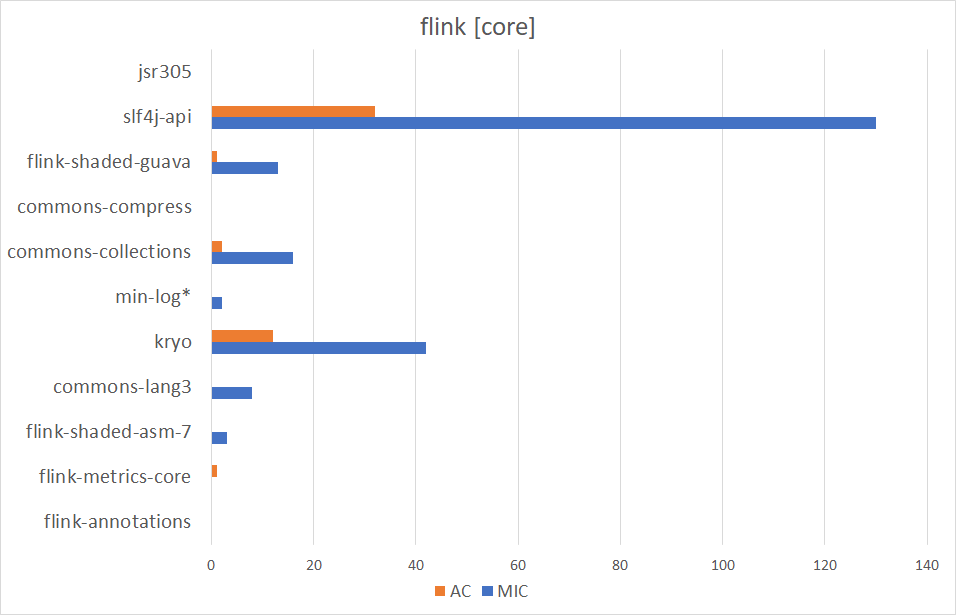
\includegraphics[width=\linewidth]{img/flink-core-excel.png}
\caption{Results of \texttt{MIC} and \texttt{AC} for library \texttt{flink-core}}
\label{fig:flink-core}
\end{center}
\end{figure}
%
%For some transitive dependencies, there is coupling measured by \texttt{MIC} and/or \texttt{AC}. In Figure \ref{fig:flink-core} \texttt{min-log} is a transitive dependency (marked with an asterisk). This indicates that the client library directly uses the transitive dependency. This could be due to the fact that our implementation determines the class in which the method is implemented. Therefore, it could happen that a direct dependency inherits a method from another library, and this is the method used by the client library.

%When comparing the two metrics, we have found that
Most of the dependencies that have $\verb|AC| \neq 0$ also have $\verb|MIC| \neq 0$. Figure~\ref{fig:flink-core} shows a single case of a dependency (\texttt{flink-metrics-core}) that has $\verb|AC| = 1$ and $\verb|MIC| = 0$ %(dependency \texttt{flink-metrics-core} in Figure \ref{fig:flink-core}).
There are also cases where a dependency has $\verb|MIC| > 0$ and $\verb|AC| = 0$.

Figure \ref{fig:flink-core} shows that the values of \texttt{MIC} range from 0 to 130, and \texttt{AC} from 0 to 32. However, for some other libraries that were investigated (but not shown here) this range is greater. For example, the \texttt{MIC} ranges from zero to 7212 for \texttt{puppycrawl-tools-checkstyle}.

\section{Conclusion and Next Steps}
%With this initial research, we defined the first two metrics to measure the degree of library dependency.
We leveraged the framework defined by Briand et al. to formulate the definition of coupling to be measured. The framework was adapted to the use case of dependencies between libraries. The result is the definition of two metrics which measure different types of connection between libraries: method invocations and aggregation. An initial proof-of-concept (PoC) has been implemented and used with some example libraries.

We plan to extend the work presented by defining the metrics to measure transitive dependencies. Next, we will perform the theoretical validation of the metrics based on the properties defined by Briand et al. In addition, we will improve the PoC tool to calculate and compare the metrics defined.

%The PoC will use versioned call-level graphs, to obtain precise %and fine-grained data.

Then, we will focus on the second research question. We will study different cases of dependency replacement, how it affects a code and how much effort is required for the replacement.
%and %how each of these cases affect a project.
%for each case, we will determine how it affects the code.
Finally, we will %validate the proposed method by
compare the real effort invested in a replacement with the effort estimated by our model.

\section{Acknowledgment}
The work of the second author on this paper has been executed with the scope of the FASTEN project. The FASTEN project has received funding from the European Union's Horizon 2020 research and innovation programme under grant agreement No 825328.

\bibliographystyle{alpha}
\bibliography{res}
%inline the .bbl file directly for mailing to authors.

\end{document}
